\documentclass{templateNote}
\usepackage{tcolorbox}
\usepackage{svg}
\usepackage{amssymb}
\usepackage{pgfplots}
\usepackage{tikz}
\usepackage{soul}
\usepackage{amsmath}
\usepackage{xcolor}
\usepackage{graphicx}
\usepackage{hyperref}

\usetikzlibrary{tikzmark,calc}

\pgfplotsset{compat=1.18}

\newcommand{\destacar}[1]{ \colorbox{yellow}{#1}}
\newcommand{\hlblue}[1]{{\sethlcolor{blue!20!white}\hl{#1}}}
\newcommand{\hlgreen}[1]{{\sethlcolor{green!20!white}\hl{#1}}}

\begin{document}

\imagenlogoU{img/LogoElNube.png}
\linklogoU{https://github.com/MarceloPazPezo}
\linkDoc{https://github.com/MarceloPazPezo/MyRepo/blob/main/Icinf/Semestre\%206/Base\%20de\%20Datos/Teoria/ApunteC3/ApunteC3.pdf}
\universidad{Universidad del Bío-Bío}
\titulo{Apunte Certamen 3} % Titulo
\asignatura{Base de Datos} % Asignatura
\autor{
    Marcelo \textsc{Paz}
}
\portada
\margenes % Crear márgenes

\section{Importante}

\begin{itemize}
    \item \textbf{Dependencia Funcional:} Sea $r$ una relación $y$ $X,Y \subseteq R$ entonces $X \rightarrow Y$ es una dependencia funcional de $r$ si y solo si para cada par de tuplas $t_1$ y $t_2$ de $r$ si $t_1[X] = t_2[X]$ entonces $t_1[Y] = t_2[Y]$.  
    \textbf{\href{https://www.youtube.com/watch?v=1PJLDStZVlo}{Video explicativo}}

    Ejercicio:
    \begin{center}
        \begin{tabular}{|c|c|c|c|}
            \hline
            \textbf{A} & \textbf{B} & \textbf{C} & \textbf{D} \\ \hline
            $a_1$ & $b_1$ & $c_1$ & $d_1$ \\ \hline
            $a_1$ & $b_2$ & $c_1$ & $d_2$ \\ \hline
            $a_2$ & $b_2$ & $c_2$ & $d_2$ \\ \hline
            $a_2$ & $b_3$ & $c_2$ & $d_3$ \\ \hline
            $a_3$ & $b_3$ & $c_2$ & $d_4$ \\ \hline
        \end{tabular}
    \end{center}

    DF trivial $ A \rightarrow A$
    \begin{center}
        
        \begin{minipage}{0.3\textwidth}
            1. $A \rightarrow C$
            \\

            \centering
            \begin{tabular}{|c|c|}
                \hline
                \textbf{A} & \textbf{C} \\ \hline
                $a_1$ & $c_1$ \\ \hline
                $a_1$ & $c_1$ \\ \hline
                $a_2$ & $c_2$ \\ \hline
                $a_2$ & $c_2$ \\ \hline
                $a_3$ & $c_2$ \\ \hline
            \end{tabular}
        \end{minipage}
        % \hfill
        \begin{minipage}{0.3\textwidth}
            2. $C \rightarrow A$
            \\

            \centering
            \begin{tabular}{|c|c|}
                \hline
                \textbf{C} & \textbf{A} \\ \hline
                $c_1$ & $a_1$ \\ \hline
                $c_1$ & $a_1$ \\ \hline
                \rowcolor{red!20!white} $c_2$ & $a_2$ \\ \hline
                \rowcolor{red!20!white} $c_2$ & $a_2$ \\ \hline
                \rowcolor{red!20!white} $c_2$ & $a_3$ \\ \hline
            \end{tabular}
        \end{minipage}
        % \hfill
        \begin{minipage}{0.3\textwidth}
            3. $AB \rightarrow D$
            \\

            \centering
            \begin{tabular}{|c|c|}
                \hline
                \textbf{AB} & \textbf{D} \\ \hline
                $a_1b_1$ & $d_1$ \\ \hline
                $a_1b_2$ & $d_2$ \\ \hline
                $a_2b_2$ & $d_2$ \\ \hline
                $a_2b_3$ & $d_3$ \\ \hline
                $a_3b_3$ & $d_4$ \\ \hline
            \end{tabular}
        \end{minipage}
    \end{center}

    
    \item \textbf{Leyes de Armstrong S+:} Sean $A,B,C,D \subseteq R$ y $r$ una relación.
    \begin{enumerate}
        \item \textit{Reflexibilidad:} Si $B \subset A$ / $A \rightarrow B$.
        \item \textit{Aumentatividad:} $A \rightarrow B$ / C \qquad $AC \rightarrow BC$.
        \item \textit{Descomposición:} $A \rightarrow BC$ \qquad $A \rightarrow B \wedge A \rightarrow C$.
        \item \textit{Composición:} $A \rightarrow B$ $\wedge$ $C \rightarrow D$ \qquad $AC \rightarrow BD$.
        \item \textit{Autodeterminación:} $A \rightarrow A$.
        \item \textit{*Transitividad:} $A \rightarrow B$ $\wedge$ $B \rightarrow C$ \qquad $A \rightarrow C$.
        \item \textit{Pseudotransitividad:} $A \rightarrow B \wedge CB \rightarrow D$ \qquad $AC \rightarrow D$.
    \end{enumerate}

    \newpage
    \item \textbf{Super Clave:} Un atributo que determina al resto. Es aquella que es determinante para todos los atributos.

    \item \textbf{Clave Candidata:} Sea $r$ una relación y $X \subseteq R$ es una clave candidata de $r$ si y solo si $X \rightarrow R$ y $X$ es minimal.
    \textbf{\href{https://www.youtube.com/watch?v=MRD35wGmsUg}{Video algoritmo alternativo}}

    \item \textbf{Forma Normal:} Es una propiedad que satisface un cierto número de restricciones para tener una buena optimización.
    \textbf{\href{https://www.youtube.com/playlist?list=PLE19WVM4rff1ion43QTNdbbejTKNhYs8x}{Video explicativo}}
    
    \begin{enumerate}
        \item \textbf{1FN:} Todos los atributos son atómicos y posee alguna clave candidata.
        \\

        \begin{minipage}{0.5\textwidth}
            \begin{tabular}{|c|}
                \hline
                \textbf{Nombre}\\ \hline
                \rowcolor{red!20!white} Marcelo Paz \\ \hline
            \end{tabular}
        \end{minipage}
        \hfill
        \begin{minipage}{0.5\textwidth}
            \begin{tabular}{|c|c|}
                \hline
                \textbf{Nombre} & \textbf{Apellido}\\ \hline
                \rowcolor{green!20!white} Marcelo & Paz \\ \hline
            \end{tabular}
        \end{minipage}
        \\
        
        \item \textbf{2FN:} Está en 1FN y todos los atributos no primos dependen de la clave candidata(los atributos depende de su clave).
        
        Sea $R(A,B,C,D,F)$ con DFs:
        \begin{itemize}
            \item $AB \rightarrow C$
            \item $AB \rightarrow D$
            \item $AB \rightarrow E$
            \item $E \rightarrow F$
        \end{itemize}

        \begin{figure}[H]
            \centering
            \colorbox{green!20!white}{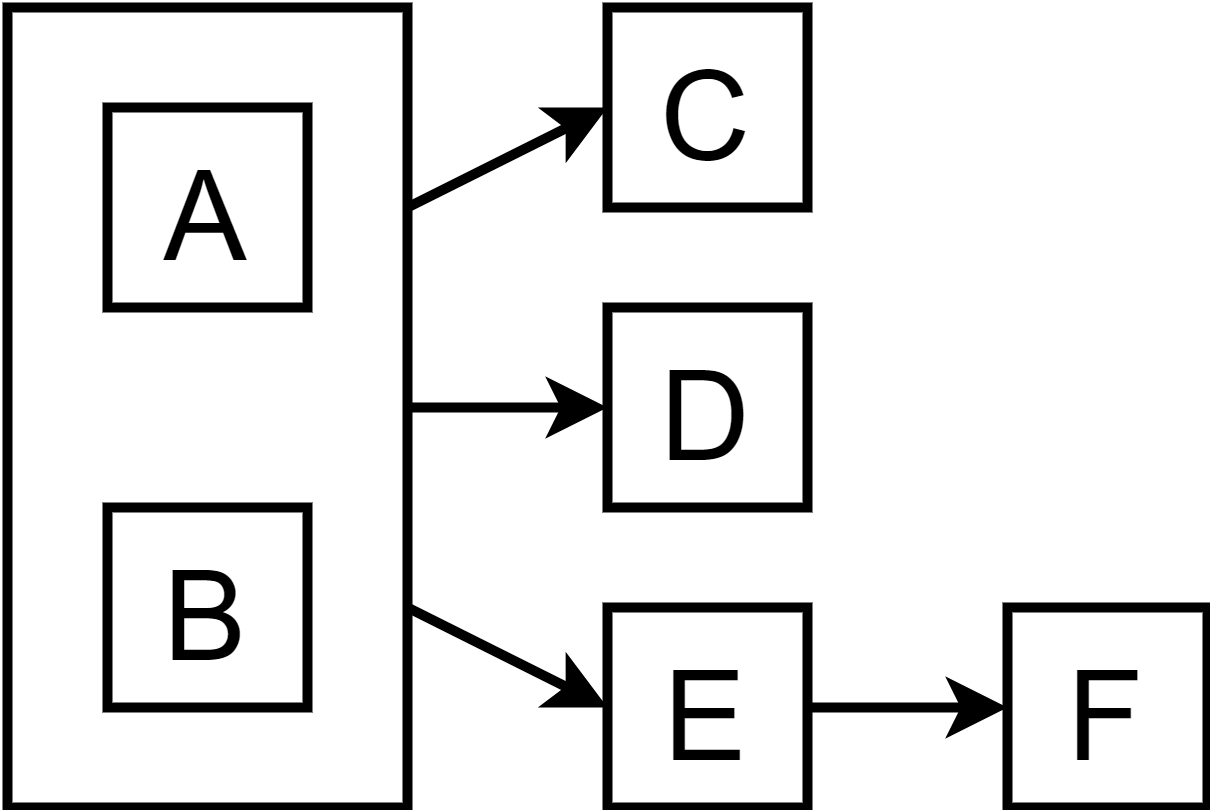
\includegraphics[scale=0.08]{img/2FN.png}}
        \end{figure}

        R está en 2FN porque $C$, $D$ y $E$ dependen de la clave candidata $AB$ y $F$ depende transitivamente de $AB$.
        
        Sea $R(A,B,C,D,F)$ con DFs:
        \begin{itemize}
            \item $AB \rightarrow C$
            \item $AB \rightarrow D$
            \item $B \rightarrow E$
            \item $E \rightarrow F$
        \end{itemize}

        \begin{figure}[H]
            \centering
            \colorbox{red!20!white}{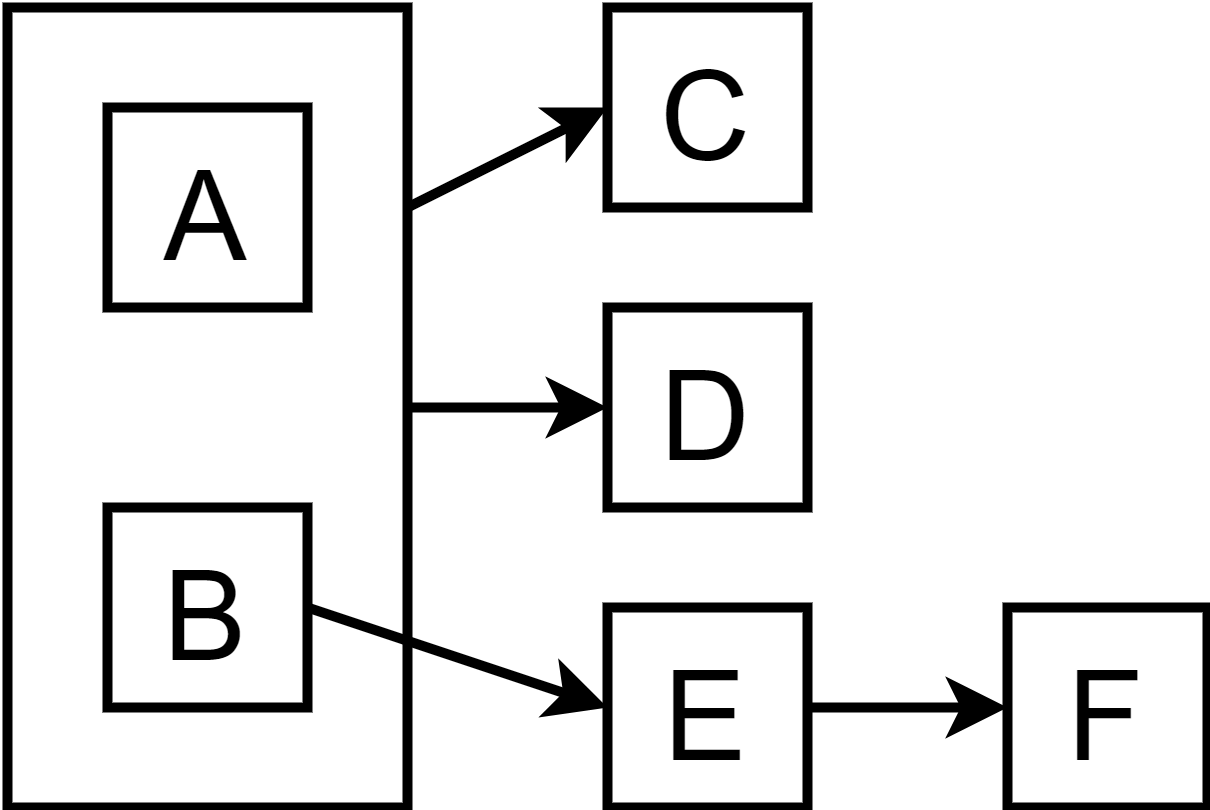
\includegraphics[scale=0.08]{img/NO2FN.png}}
        \end{figure}
        R NO está en 2FN porque $E$ depende de $B$.

        Descomposición a 2FN:
        \begin{itemize}
            \item $R_1(B,E,F)$
            \item $R_2(A,B,C,D)$
        \end{itemize}

        \newpage
        \item \textbf{3FN:} Está en 2FN y cada atributo no clave depende de manera no transitiva de atributos clave.
        
        
        Sea $R(A,B,C,D,E)$ con DFs:
        \begin{itemize}
            \item $AB \rightarrow C$
            \item $AB \rightarrow D$
            \item $AB \rightarrow E$
        \end{itemize}

        \begin{figure}[H]
            \centering
            \colorbox{green!20!white}{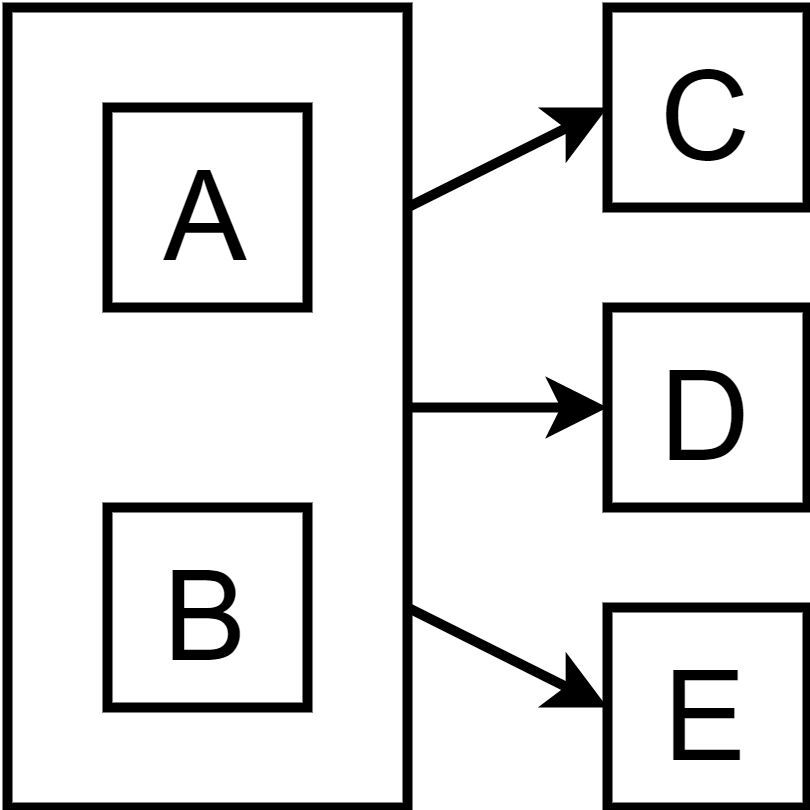
\includegraphics[scale=0.08]{img/3FN.png}}
        \end{figure}

        R está en 3FN porque $C$, $D$ y $E$ dependen de la clave candidata $AB$.
        
        Sea $R(A,B,C,D,E)$ con DFs:
        \begin{itemize}
            \item $AB \rightarrow C$
            \item $AB \rightarrow D$
            \item $D \rightarrow E$
        \end{itemize}

        \begin{figure}[H]
            \centering
            \colorbox{red!20!white}{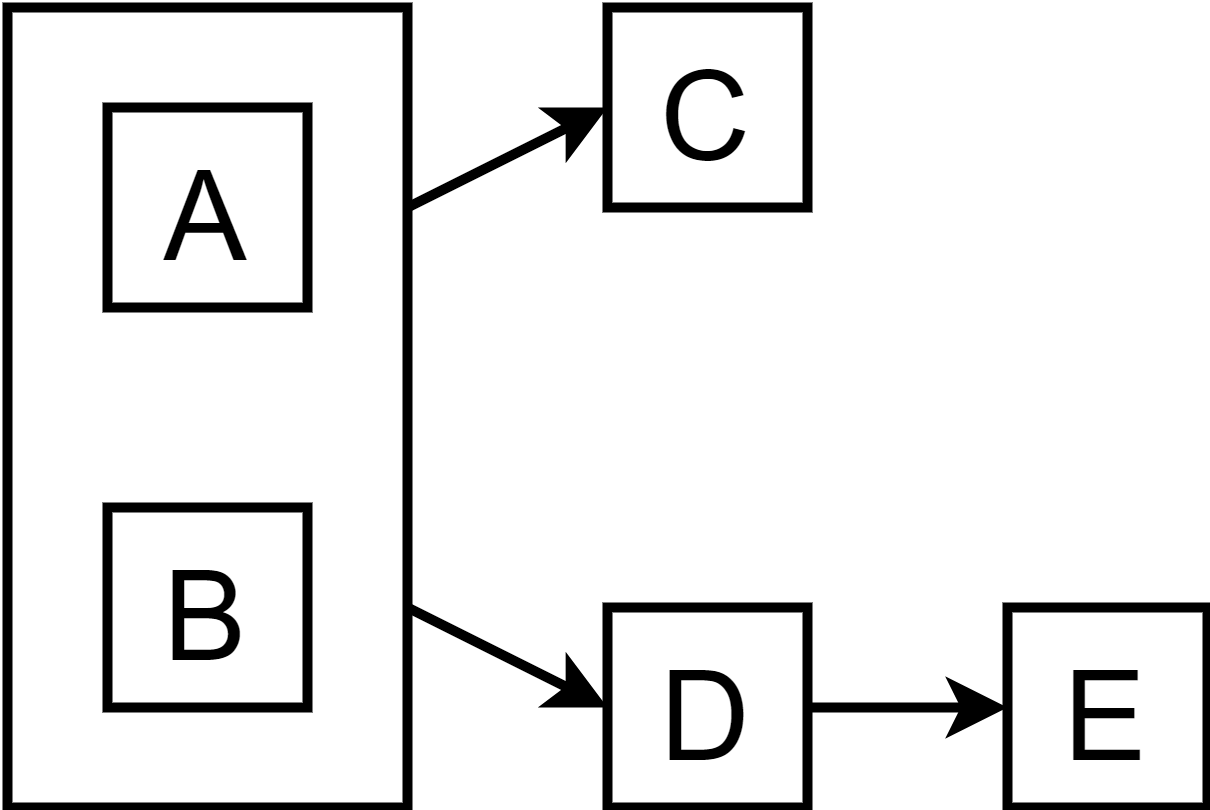
\includegraphics[scale=0.08]{img/NO3FN.png}}
        \end{figure}

        R NO está en 3FN porque $E$ depende transitivamente de $AB$.

        Descomposición a 3FN:
        \begin{itemize}
            \item $R_1(D,E)$
            \item $R_2(A,B,C,D)$
        \end{itemize}
        
        \item \textbf{FNBC:} Está en 3FN y existen dos o más llaves candidatas para la relación, éstas son llaves compuestas (con más de un atributo) y su intersección no es vacía.
        
        \begin{minipage}{0.4\textwidth}
            \begin{center}
                Sea $R(A,B,C,D,E)$ con DFs:
                \begin{itemize}
                    \item $AB \rightarrow CDE$
                    \item $C \rightarrow A$
                \end{itemize}
                \begin{figure}[H]
                    \centering
                    \colorbox{red!20!white}{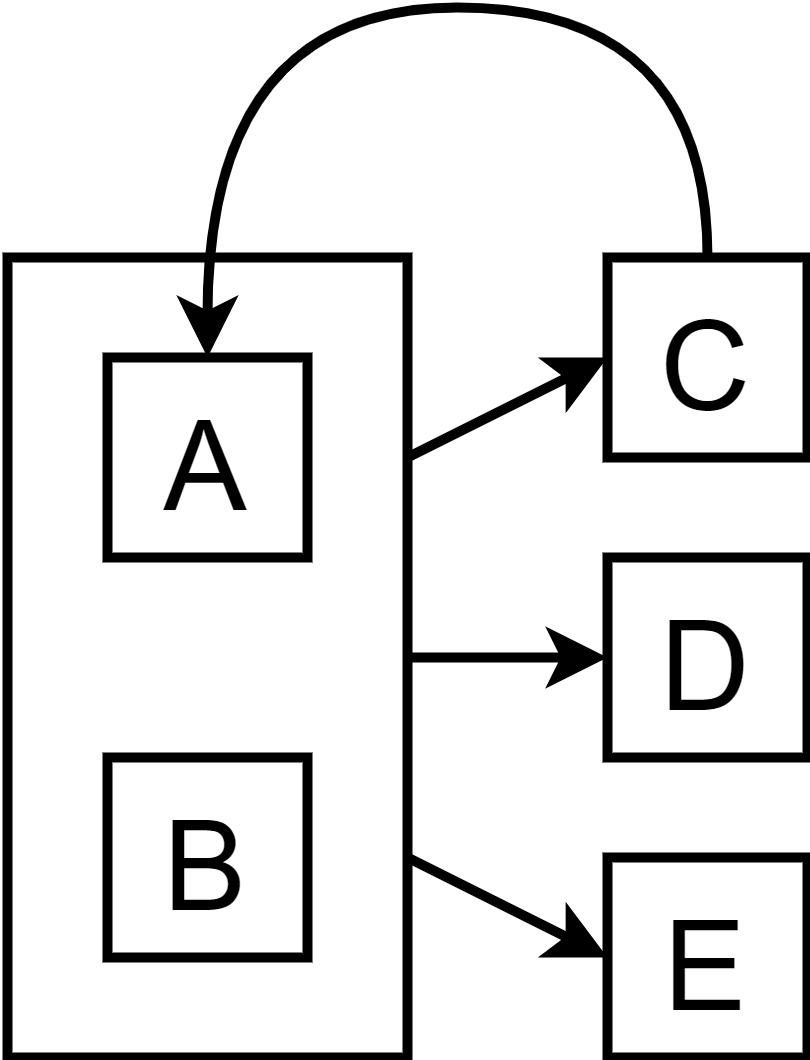
\includegraphics[scale=0.08]{img/NOFNBC.png}}
                \end{figure}

                R NO está en FNBC porque $C$ depende de $A$ y $A$ no es clave.
            \end{center}
        \end{minipage}
        \vline
        \begin{minipage}{0.4\textwidth}
            \begin{center}
                Sea $R(A,B,C,D,E)$ con DFs:
                \begin{itemize}
                    \item $AB \rightarrow CDE$
                \end{itemize}
                \begin{figure}[H]
                    \centering
                    \colorbox{green!20!white}{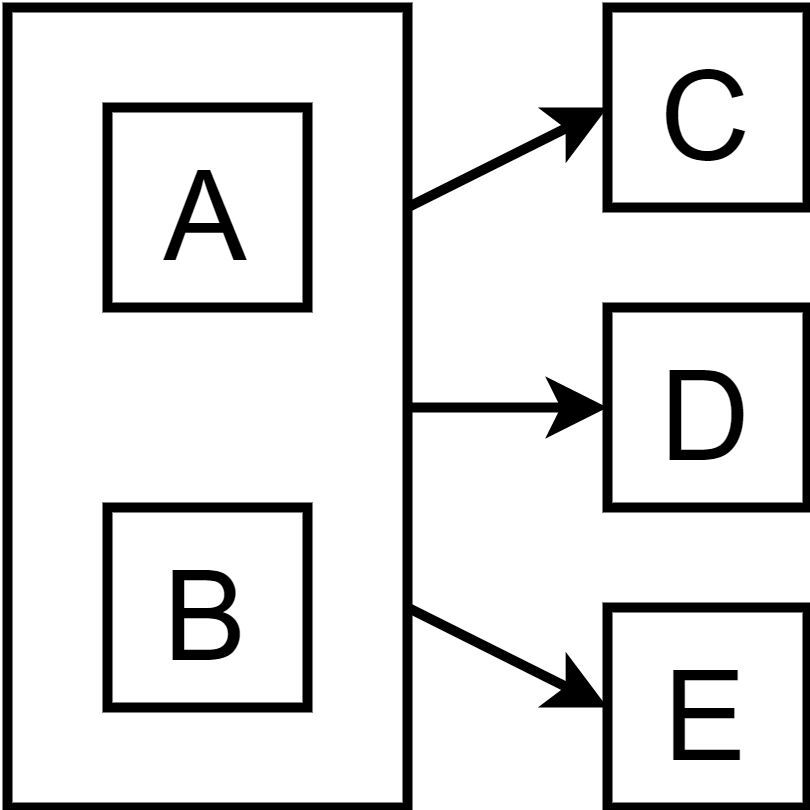
\includegraphics[scale=0.08]{img/FNBC.png}}
                \end{figure}
                R está en FNBC porque $AB$ es clave.
            \end{center}
        \end{minipage}
        
    \end{enumerate}

    \newpage
    \item \textbf{Transacciones:}Las transacciones son el fundamento de le ejecución concurrente y la recuperación de un fallo del sistema en un SGBD
    
    \item \textbf{SGBD}:Sistemas Gestores de Base de Datos son la opción perfecta para crear, gestionar y administrar las bases de datos que poseas.
    
    Desde el punto de vista de SGBD, una transacción es una serie de operaciones de escritura y lectura a la BD.

    Propiedades:
    \begin{enumerate}
        \item La ejecución de cada transacción es atómica: o se realizan todas las acciones o no se realiza ninguna.
        \item Consistencia: las transacciones deben preservar la consistencia de la BD.
        \item Aislamiento: las transacciones están aisladas, o protegidas, de los efectos de otras transacciones.
        \item Durabilidad: si la transacción finaliza exitosamente, sus efectos deben persistir incluso si se produce una caída del sistema.
    \end{enumerate}

    Acciones:
    \begin{itemize}
        \item \textbf{$R_t(O)$} denota lectura del objeto $O$ por transacción $t$.
        \item \textbf{$W_t(O)$} denota escritura de $O$ por $t$.
        \item \textbf{Commit(comprometer)} indica que la transacción está terminada satisfactoriamente.
        \item \textbf{Abort(abortar)} indica que la transacción está terminada y deshechos los cambios realizados en la BD.
    \end{itemize}

    \item \textbf{Plan de ejecución:} es una lista de acciones (lectura, escritura, comprometer o abortar) de un conjunto de transacciones.

    Tipo de plan:
    \begin{itemize}
        \item \textbf{Plan serial(Secuenciable):} es aquel en el que las transacciones son ejecutadas de inicio a fin, una por una.
        \begin{figure}[H]
            \centering
            \begin{tabular}{|c|c|}
                \hline
                \multicolumn{2}{|c|}{\textbf{Serial: $T_1 \rightarrow T_2$}} \\ \hline
                \textbf{$T_1$} & \textbf{$T_2$} \\ \hline
                \textcolor{blue}{$R(A)$} & \\
                \textcolor{blue}{$W(A)$} & \\
                \textcolor{blue}{$R(C)$} & \\
                \textcolor{blue}{$W(C)$} & \\
                \textcolor{blue}{\textit{$commit_{T_1}$}} & \\ \hline
                & \textcolor{green!80!black}{$R(B)$} \\
                & \textcolor{green!80!black}{$W(B)$} \\
                & \textcolor{green!80!black}{\textit{$commit_{T_2}$}} \\ \hline
            \end{tabular}
        \end{figure}

        \newpage
        Conflictos:
        \begin{itemize}
            \item \textbf{Escritura-Lectura (WR):} Lectura sucia. $T_2$ lee un objeto que fue modificado por $T_1$, pero que aún no ha sido comprometido.
            
            Sea: A = 1000 y B = 500.
            
            \subitem $T_1$ transfiere 100 desde A a B.
            
            \subitem $T_2$ incrementa A y B en 10\%.

            \begin{figure}[H]
                \centering
                \begin{minipage}{0.3\textwidth}
                    \resizebox{\textwidth}{!}{
                    \begin{tabular}{|c|c|}
                        \hline
                        \multicolumn{2}{|c|}{\textbf{WR}} \\ \hline
                        \textbf{$T_1$} & \textbf{$T_2$} \\ \hline
                        \textcolor{blue}{$R(A), A = 1000$} & \\
                        \textcolor{blue}{$W(A), A = 900$} & \\ \hline
                        & \textcolor{green!80!black}{$R(A), A = 900$} \\
                        & \textcolor{green!80!black}{$W(A), A = 990$} \\
                        & \textcolor{green!80!black}{$R(B), B = 500$} \\
                        & \textcolor{green!80!black}{$W(B), B = 550$} \\
                        & \textcolor{green!80!black}{\textit{$commit_{T_2}$}} \\ \hline
                        \textcolor{blue}{$R(B), B = 550$} & \\
                        \textcolor{blue}{$W(B), B = 650$} & \\
                        \textcolor{blue}{\textit{$commit_{T_1}$}} & \\ \hline
                        \multicolumn{2}{|c|}{$A = 990$ y $B = 650$.} \\ \hline
                    \end{tabular}
                    }
                \end{minipage}
                \begin{minipage}{0.3\textwidth}
                    \resizebox{\textwidth}{!}{
                    \begin{tabular}{|c|c|}
                        \hline
                        \multicolumn{2}{|c|}{\textbf{$T_1 \rightarrow T_2$}} \\ \hline
                        \textbf{$T_1$} & \textbf{$T_2$} \\ \hline
                        \textcolor{blue}{$R(A), A = 1000$} & \\
                        \textcolor{blue}{$W(A), A = 900$} & \\
                        \textcolor{blue}{$R(B), B = 500$} & \\
                        \textcolor{blue}{$W(B), B = 600$} & \\
                        \textcolor{blue}{\textit{$commit_{T_1}$}} & \\ \hline
                        & \textcolor{green!80!black}{$R(A), A = 900$} \\
                        & \textcolor{green!80!black}{$W(A), A = 990$} \\
                        & \textcolor{green!80!black}{$R(B), B = 600$} \\
                        & \textcolor{green!80!black}{$W(B), B = 660$} \\
                        & \textcolor{green!80!black}{\textit{$commit_{T_2}$}} \\ \hline
                        \multicolumn{2}{|c|}{$A = 990$ y $B = 660$.} \\ \hline
                    \end{tabular}
                    }
                \end{minipage}
                \begin{minipage}{0.3\textwidth}
                    \resizebox{\textwidth}{!}{
                    \begin{tabular}{|c|c|}
                        \hline
                        \multicolumn{2}{|c|}{\textbf{$T_2 \rightarrow T_1$}} \\ \hline
                        \textbf{$T_1$} & \textbf{$T_2$} \\ \hline
                        & \textcolor{green!80!black}{$R(A), A = 1000$} \\
                        & \textcolor{green!80!black}{$W(A), A = 1100$} \\
                        & \textcolor{green!80!black}{$R(B), B = 500$} \\
                        & \textcolor{green!80!black}{$W(B), B = 550$} \\
                        & \textcolor{green!80!black}{\textit{$commit_{T_2}$}} \\ \hline
                        \textcolor{blue}{$R(A), A = 1100$} & \\
                        \textcolor{blue}{$W(A), A = 1000$} & \\
                        \textcolor{blue}{$R(B), B = 550$} & \\
                        \textcolor{blue}{$W(B), B = 650$} & \\
                        \textcolor{blue}{\textit{$commit_{T_1}$}} & \\ \hline
                        \multicolumn{2}{|c|}{$A = 1000$ y $B = 650$.} \\ \hline
                    \end{tabular}
                    }
                \end{minipage}
            \end{figure}

            El problema es que $T_2$ lee el valor de A modificado por $T_1$ pero no comprometido. Mostrándonos resultados diferentes.

            \item \textbf{Lectura-Escritura(RW):} $T_2$ modifica el valor de un objeto A que es leído por una $T_1$, mientras $T_1$ está áun en progreso.
            
            Considere las transacciones $T_1$ y $T_2$, y sea A el número de copias disponibles de un libro.
            \subitem $T_1$ lee A = 1.
            \subitem $T_2$ lee A = 1, resta 1 y compromete (A=0)
            
            T1 trata de restar 1 a A y recibe un error, A ya no tiene el valor 1
            
            \item \textbf{Escritura-Escritura(WW):} $T_2$ sobrescribe el valor de un objeto A que ya ha sido modificado por una transacción $T_1$, mientras $T_1$ todavía está en progreso.
            
            Suponga que los salario de Pedro y Juan deben ser iguales:
            \subitem $T_1$ asigna salarios iguales a 2000.
            \subitem $T_2$ asigna salarios iguales a 1000.

            \begin{figure}[H]
                \centering
                \begin{tabular}{|c|c|}
                    \hline
                    \textbf{$T_1$} & \textbf{$T_2$} \\ \hline
                    & \textcolor{green!80!black}{$W(Pedro), Salario = 1000$} \\
                    \textcolor{blue}{$W(Juan), Salario = 2000$} & \\
                    & \textcolor{green!80!black}{$W(Juan), Salario = 1000$} \\
                    & \textcolor{green!80!black}{\textit{$commit_{T_2}$}} \\
                    \textcolor{blue}{$W(Pedro), Salario = 2000$} & \\
                    \textcolor{blue}{\textit{$commit_{T_1}$}} & \\ \hline
                    \multicolumn{2}{|c|}{$P_{salario} \neq J_{salario}$} \\ \hline
                \end{tabular}
            \end{figure}
        \end{itemize}

        \newpage
        \item \textbf{Plan con Abort:} Cuando una transacción aborta, todas las acciones son deshechas, y la BD vuelve al estado inicial.
        
        Considere las transacciones $T_1$ y $T_2$:
        \subitem $T_1$ transfiere 100 desde la cuenta A a la B.
        \subitem $T_2$ incrementa A y B por el 10\%.
        
        Supongamos los valores iniciales A = 1000 y B = 500
         
        \begin{figure}[H]
            \centering
            \begin{tabular}{|c|c|}
                \hline
                \textbf{$T_1$} & \textbf{$T_2$} \\ \hline
                \textcolor{blue}{$R(A), A = 1000$} & \\
                \textcolor{blue}{$W(A), A = 900$} & \\
                & \textcolor{green!80!black}{$R(A), A = 900$} \\
                & \textcolor{green!80!black}{$W(A), A = 990$} \\
                & \textcolor{green!80!black}{$R(B), B = 500$} \\
                & \textcolor{green!80!black}{$W(B), B = 550$} \\
                & \textcolor{green!80!black}{\textit{$commit_{T_2}$}} \\
                \textcolor{blue}{$abort_{T_t}$} & \\ \hline
            \end{tabular}
        \end{figure}

        $T_2$ ha ha leído un valor de A que no debería haber estado nunca ahí.

        Como $T_2$ ya comprometió sus acciones no pueden ser deshechas

        \item \textbf{Plan recuperable:} las transacciones se comprometen sólo después de que se comprometan a su vez todas las transacciones que hayan leído sus cambios.
        
        \item \textbf{Planes conflictos equivalentes:} Dos acciones están en conflicto si operan sobre el mismo objeto y al menos una de ellas es escritura.
        
        Podemos cambiar el orden de acciones que no son conflictivas sin alterar el efecto del plan sobre la BD
        
        Todo plan conflicto equivalente es serializable.

        Considere el siguiente plan:
        \begin{align*}
            R_{T_1}(x), R_{T_2}(y), W_{T_3}(x), R_{T_2}(x), R_{T_1}(y)
        \end{align*}

        \begin{figure}[H]
            \begin{minipage}{0.5\textwidth}
                \centering
                \begin{tabular}{|c|c|c|}
                    \hline
                    \textbf{$T_1$} & \textbf{$T_2$} & \textbf{$T_3$} \\ \hline
                    \textcolor{blue}{$R(x)$} & & \\
                    & \textcolor{green!80!black}{$R(y)$} & \\
                    & & \textcolor{red}{$W(x)$} \\
                    & \textcolor{green!80!black}{$R(x)$} & \\
                    \textcolor{blue}{$R(y)$} & & \\ \hline
                \end{tabular}
            \end{minipage}
            $\Rightarrow$
            \begin{minipage}{0.5\textwidth}
                \centering
                \begin{tabular}{|c|c|c|}
                    \hline
                    \textbf{$T_1$} & \textbf{$T_2$} & \textbf{$T_3$} \\ \hline
                    \textcolor{blue}{$R(x)$} & & \\
                    \textcolor{blue}{$R(y)$} & & \\
                    & & \textcolor{red}{$W(x)$} \\
                    & \textcolor{green!80!black}{$R(y)$} & \\
                    & \textcolor{green!80!black}{$R(x)$} & \\ \hline
                \end{tabular}
            \end{minipage}
        \end{figure}

        \begin{enumerate}
            \item Las lecturas de $T_1$ pueden ser ejecutadas en el siguiente orden:
            
            \textcolor{blue}{$R_{T_1}(x), R_{T_1}(y),$} $R_{T_2}(y), W_{T_3}(x), R_{T_2}(x)$

            \item La lectura de $T_2$ se puede reordenar de la siguiente forma:
            
            \textcolor{blue}{$R_{T_1}(x), R_{T_2}(y),$} \textcolor{red}{$W_{T_3}(x),$}\textcolor{green!80!black}{$R_{T_2}(x), R_{T_1}(y)$}

            \item El plan es conflicto equivalente a la ejecución serial $T_1$-$T_3$-$T_2$, y como consecuencia el plan es serializable.
        \end{enumerate}
    \end{itemize}

    \item \textbf{Control de Concurrencia Basado en Bloqueos:} Un SGBD solo debe permitir la ejecución de planes que son
    serializables y recuperables.
    
    Tipos de bloqueos:
    \begin{itemize}
        \item \textbf{Bloqueo compartido ($S_T(O)$):} Un bloqueo compartido sobre un objeto $O$ permite que una transacción $T$ lea $O$ pero no lo modifique.

        \item \textbf{Bloqueo exclusivo ($X_T(O)$):} Un bloqueo exclusivo sobre un objeto $O$ permite que una transacción $T$ lea y modifique $O$.
    \end{itemize}

    Protocolos:
    \begin{itemize}
        \item \textbf{2PL estricto:} El protocolo 2PL estricto permite que solo planes seguros sean ejecutados.

        Reglas:
        \begin{enumerate}
            \item Si una transacción T quiere leer (respectivamente, modificar) un objeto, primero solicita un bloqueo compartido (respectivamente, exclusivo) sobre el objeto.
            
            \item Todos los bloqueos concedidos a una transacción se liberan cuando la transacción se completa.
        \end{enumerate}

        \begin{figure}[H]
            \begin{minipage}{0.5\textwidth}
                \centering
                \colorbox{green!20!white}{
                \begin{tabular}{|c|c|}
                    \hline
                    \textbf{$T_1$} & \textbf{$T_2$} \\ \hline
                    \textcolor{blue}{$X(A)$} & \\
                    \textcolor{blue}{$R(A)$} & \\
                    \textcolor{blue}{$W(A)$} & \\
                    \textcolor{blue}{$X(B)$} & \\
                    \textcolor{blue}{$R(B)$} & \\
                    \textcolor{blue}{$W(B)$} & \\
                    \textcolor{blue}{\textit{$commit_{T_1}$}} & \\ \hline
                    & \textcolor{green!80!black}{$X(B)$} \\
                    & \textcolor{green!80!black}{$R(B)$} \\
                    & \textcolor{green!80!black}{$W(B)$} \\
                    & \textcolor{green!80!black}{\textit{$commit_{T_2}$}} \\ \hline
                \end{tabular}
                }
            \end{minipage}
            \hfill
            \begin{minipage}{0.5\textwidth}
                \centering
                \colorbox{green!20!white}{
                \begin{tabular}{|c|c|}
                    \hline
                    \textbf{$T_1$} & \textbf{$T_2$} \\ \hline
                    \textcolor{blue}{$S(A)$} & \\
                    \textcolor{blue}{$R(A)$} & \\
                    & \textcolor{green!80!black}{$S(A)$} \\
                    & \textcolor{green!80!black}{$R(A)$} \\
                    & \textcolor{green!80!black}{$X(B)$} \\
                    & \textcolor{green!80!black}{$R(B)$} \\
                    & \textcolor{green!80!black}{$W(B)$} \\
                    & \textcolor{green!80!black}{\textit{$commit_{T_2}$}} \\ \hline
                    \textcolor{blue}{$X(C)$} & \\
                    \textcolor{blue}{$R(C)$} & \\
                    \textcolor{blue}{$W(C)$} & \\
                    \textcolor{blue}{\textit{$commit_{T_1}$}} & \\ \hline
                \end{tabular}
                }
            \end{minipage}

            \vspace{0.5cm}

            \begin{center}
                \colorbox{red!20!white}{
                \begin{tabular}{|c|c|}
                    \hline
                    \textbf{$T_1$} & \textbf{$T_2$} \\ \hline
                    \textcolor{blue}{$R(A)$} & \\
                    \textcolor{blue}{$W(A)$} & \\
                    & \textcolor{green!80!black}{$R(A)$} \\
                    & \textcolor{green!80!black}{$W(A)$} \\
                    & \textcolor{green!80!black}{$R(B)$} \\
                    & \textcolor{green!80!black}{$W(B)$} \\
                    & \textcolor{green!80!black}{\textit{$commit_{T_2}$}} \\ \hline
                    \textcolor{blue}{$R(B)$} & \\
                    \textcolor{blue}{$W(B)$} & \\
                    \textcolor{blue}{\textit{$commit_{T_1}$}} & \\ \hline
                \end{tabular}
                }
            \end{center}

        \end{figure}



        \newpage
        \item \textbf{2PL:} En 2PL una transacción puede entregar sus candados antes del final de la transacción (antes de commit o abort).

        Reglas:
        \begin{enumerate}
            \item Si una transacción T quiere leer (respectivamente, modificar) un objeto, primero solicita un bloqueo compartido (respectivamente, exclusivo) sobre el objeto.
            
            \item Una transacción no puede pedir candados adicionales una vez que empieza a devolver sus candados.
        \end{enumerate}

        \begin{figure}[H]
            \centering
            \begin{tabular}{|c|c|}
                \hline
                \textbf{$T_1$} & \textbf{$T_2$} \\ \hline
                \textcolor{blue}{$X(A)$} & \\
                \textcolor{blue}{$R(A)$} & \\
                \textcolor{blue}{$W(A)$} & \\
                \textcolor{blue}{$X(B)$} & \\
                \textcolor{blue}{\textit{$liberar{X(A)}$}} & \\
                & \textcolor{green!80!black}{$X(A)$} \\
                & \textcolor{green!80!black}{$R(A)$} \\
                & \textcolor{green!80!black}{$W(A)$} \\
                & \textcolor{green!80!black}{$X(C)$} \\
                & \textcolor{green!80!black}{$W(C)$} \\
                & \textcolor{green!80!black}{\textit{$liberar{X(A)}$}} \\
                & \textcolor{green!80!black}{\textit{$liberar{X(C)}$}} \\
                & \textcolor{green!80!black}{\textit{$commit_{T_2}$}} \\ \hline
                \textcolor{blue}{$W(B)$} & \\
                \textcolor{blue}{\textit{$liberar{X(B)}$}} & \\
                \textcolor{blue}{\textit{$commit_{T_1}$}} & \\ \hline
            \end{tabular}
        \end{figure}
    \end{itemize}

    \item \textbf{Interbloqueos:} Es un ciclo en el cual dos o más transacción esperan por un bloqueo que la otra tiene.
    
    \begin{figure}[H]
        \centering
        \begin{tabular}{|c|c|}
            \hline
            \textbf{$T_1$} & \textbf{$T_2$} \\ \hline
            \textcolor{blue}{$X(A)$} & \\
            \textcolor{blue}{$R(A)$} & \\
            \textcolor{blue}{$W(A)$} & \\
            & \textcolor{green!80!black}{$X(B)$} \\
            & \textcolor{green!80!black}{$R(B)$} \\
            & \textcolor{green!80!black}{$W(B)$} \\
            \textcolor{blue}{\textit{$Solicita$  ${X(B)}$}} & \\
            & \textcolor{green!80!black}{\textit{$Solicita$ ${X(A)}$}} \\ \hline
        \end{tabular}
    \end{figure}

    Prevención: Se le otorga a cada transacción un \hl{nivel de prioridad}, y se le otorga el bloqueo al que tenga mayor prioridad.

    \newpage
    \item \textbf{Recuperación de una BD:} 
    
    \item \textbf{LOG:} es un historial de las acciones ejecutadas por el SGBD.
    
    Operaciones que se registran en el LOG:
    \begin{itemize}
        \item Actualizaciones a páginas: updates.
        
        \item Commit: una transacción compromete sus cambios una vez que “commit” es registrado en el LOG y éste ha sido almacenado en disco
        
        \item Abort
        
        \item End: finalización real de la transacción, se finalizan operaciones extras como borrar archivos, etc.
        
        \item Recuperación: se registran todas las actualizaciones que son deshechas debido a abortos de transacciones o fallas del sistema.
    \end{itemize}

    \item \textbf{ARIES:} Algoritmo de recuperación de una BD.
    
    Es invocado después de una caída del sistema.

    Fases:
    \begin{enumerate}
        \item Análisis: identificación de “páginas sucias”, i.e. páginas con datos que están en el buffer y no han sido escritos en disco y la identificación de las transacciones activas.

        \item Rehacer: repetir todas las acciones, partiendo desde el último punto de revisión (checkpoint) del LOG hasta dejar la BD en el mismo estado antes de la caída.

        \item Deshacer: deshacer todas las acciones de transacciones que no se comprometieron. De esta manera, la BD refleja solo las acciones de transacciones comprometidas.
    \end{enumerate}

    Ejemplo:

    \begin{figure}[H]
        \centering
        \begin{tabular}{|c|c|l|}
            \hline
            \textbf{LSN} & & \textbf{LOG} \\ \hline
            10 & - & \textcolor{green!80!black}{update: $T_1$ escribe $P5$} \\
            20 & - & \textcolor{blue}{update: $T_2$ escribe $P3$} \\
            30 & - & \textcolor{green!80!black}{$T_1$ abort} \\
            40,45 & - & \textcolor{green!80!black}{Deshacer $T_1$ LSN 10, $T_1$ end} \\
            50 & - & \textcolor{purple!50!black}{update: $T_3$ escribe $P1$} \\
            60 & - & \textcolor{blue}{update: $T_2$ escribe $P5$} \\
            & X & \textcolor{red}{CRASH, RESTART} \\
            70 & - & \textcolor{blue}{Deshacer $T_2$ LSN 60}
            \\
            80,85 & - & \textcolor{purple!50!black}{Deshacer $T_3$ LSN 50, $T_3$ end} \\
            & X & \textcolor{red}{CRASH, RESTART} \\
            90,95 & - & \textcolor{blue}{Deshacer $T_2$ LSN 20, $T_2$ end} \\ \hline
        \end{tabular}   
    \end{figure}
\end{itemize}

\newpage
\section{Ejercicios}

\section*{Certamen 2 2022}

\begin{enumerate}
    \item Considere la relación $R(A,B,C,D,E,F)$ con DFs:
    \begin{itemize}
        \item $E \rightarrow F$ \textcolor{red}{(1)}
        \item $A \rightarrow E$ \textcolor{red}{(2)}
        \item $EC \rightarrow A$ \textcolor{red}{(3)}
        \item $ABC \rightarrow D$ \textcolor{red}{(4)}
    \end{itemize}
    
    \hrulefill

    \textbf{A)} Genere las posibles claves candidatas para R. Desarrolle paso a paso nombrando los axiomas de Armstrong. TIP: Existen 2 claves candidatas.

    Para la 1° clave candidata comenzamos de $ABC$:
    \begin{align*}
        \textcolor{red}{(4)} \qquad ABC &\rightarrow D && \text{Dado} \\
        \textcolor{red}{(5)} \qquad ABC &\rightarrow A && \text{Reflexibilidad } \textcolor{red}{(4)} \\
        \textcolor{red}{(6)} \qquad ABC &\rightarrow B && \text{Reflexibilidad } \textcolor{red}{(4)} \\
        \textcolor{red}{(7)} \qquad ABC &\rightarrow C && \text{Reflexibilidad } \textcolor{red}{(4)} \\
        \textcolor{red}{(8)} \qquad ABC &\rightarrow E && \text{Transitividad de } \textcolor{red}{(5)} \wedge \textcolor{red}{(2)} \\
        \textcolor{red}{(8)} \qquad ABC &\rightarrow F && \text{Transitividad de } \textcolor{red}{(8)} \wedge \textcolor{red}{(1)} \\
    \end{align*}

    Por lo tanto $ABC$ es una clave candidata pues obtenemos $ABCDEF$.
    
    \hrulefill

    Para la 2° clave candidata comenzamos de $EC$:
    \begin{align*}
        \textcolor{red}{(3)} \qquad EC &\rightarrow A && \text{Dado} \\
        \textcolor{red}{(5)} \qquad EC &\rightarrow E && \text{Reflexibilidad } \textcolor{red}{(3)} \\
        \textcolor{red}{(6)} \qquad EC &\rightarrow C && \text{Reflexibilidad } \textcolor{red}{(3)} \\
        \textcolor{red}{(7)} \qquad EC &\rightarrow F && \text{Transitividad de } \textcolor{red}{(5)} \wedge \textcolor{red}{(1)} \\
        \textcolor{red}{(8)} \qquad BCE &\rightarrow AB && \text{Aumentatividad en } \textcolor{red}{B} \\
        \textcolor{red}{(9)} \qquad BCE &\rightarrow A && \text{Descomposición de } \textcolor{red}{(8)} \\
        \textcolor{red}{(10)} \qquad BCE &\rightarrow B && \text{Descomposición de } \textcolor{red}{(8)} \\
        \textcolor{red}{(11)} \qquad BCE &\rightarrow C && \text{Reflexibilidad de } \textcolor{red}{(8)} \\
        \textcolor{red}{(12)} \qquad BCE &\rightarrow ABC && \text{Union de } \textcolor{red}{(8)} \wedge \textcolor{red}{(11)}\\
        \textcolor{red}{(13)} \qquad BCE &\rightarrow D && \text{Transitividad de } \textcolor{red}{(12)} \wedge \textcolor{red}{(4)}\\
    \end{align*}
    
    Por lo tanto $BCE$ es una clave candidata pues obtenemos $ABCDEF$.
    
    \newpage
    \textbf{B)} ¿En cuál forma normal se encuentra R y por qué no cumple con la siguiente forma normal? Justifique.

    \textbf{Respuesta:} R se encuentra en 1FN pues todos los atributos son atómicos. R no cumple con 2FN, porque hay DFs que dependen parcialmente de la clave candidata $E \rightarrow F$.

    \hrulefill

    \textbf{C)} Si R no está en FNBC descomponga R paulatinamente hasta dejar un conjunto de relaciones en FNBC (si es posible). Justifique cada paso.

    \textbf{Respuesta:} 
    
    $R_1 (E,F)$ 
    \begin{itemize}
        \item $E \rightarrow F$
    \end{itemize}
    * $R_1$ esta en 3FN y FNBC porque E es super clave.

    $R_2 (A,B,C,D,E)$
    \begin{itemize}
        \item $A \rightarrow E$ 
        \item $EC \rightarrow A$
        \item $ABC \rightarrow D$
    \end{itemize}

    * $R_2$ esta en 3FN pero no en FNBC porque ni A ni EC son super clave.

    Descomposición $R_2$
    \begin{itemize}
        \item $R_{21}(A,E)$
        \begin{itemize}
            \item $A \rightarrow E$
        \end{itemize}

        * $R_{21}$ esta en 3FN y FNBC porque A es super clave.
        \item $R_{22}(A,B,C,D)$
        \begin{itemize}
            \item $ABC \rightarrow D$
        \end{itemize}

        * $R_{22}$ esta en 3FN y FNBC porque ABC es super clave.
    \end{itemize}

    \hrulefill

    \item Considere la relación $R(A,B,C,D)$, donde el conjunto $AB$ es clave candidata para R.
    
    \textbf{A)} ¿Qué puede concluir a raíz de que $AB$ es clave candidata para R? TIP: nombre las dependencias funcionales que se cumplen en R.
    
    \textbf{Respuesta:}
    DFs que se cumplen en R:
    \begin{itemize}
        \item $AB \rightarrow C$
        \item $AB \rightarrow D$
    \end{itemize}

    Estas DFs satisfacen R con AB como clave candidata.

    \newpage
    \textbf{B)} Agregue una dependencia funcional de tal manera que R no cumpla con la 2FN.

    \textbf{Respuesta:}

    \begin{itemize}
        \item $A \rightarrow C$
        \item $A \rightarrow D$
        \item $B \rightarrow C$
        \item $B \rightarrow D$
    \end{itemize}
    
    \hrulefill

    \item Considere el siguiente plan:
    \begin{align*}
        S = \left\{R_3(z), R_3(y), W_2(y), R_2(z), R_3(x), R_1(x), W_1(x), W_2(x)\right\}
    \end{align*}

    \hrulefill

    \textbf{A)} Demuestre que S es conflicto equivalente a un plan serial.
    
    \textbf{Respuesta:}

    $S = $ \textcolor{orange}{$R_3(z), R_3(y),$} \textcolor{green!80!black}{$W_2(y), R_2(z),$} \textcolor{orange}{$R_3(x),$} \textcolor{blue}{$R_1(x), W_1(x),$} \textcolor{green!80!black}{$W_2(x)$}
    
    \qquad \textcolor{orange}{$R_3(z), R_3(y), R_3(x),$} \textcolor{green!80!black}{$W_2(y), R_2(z),$} \textcolor{blue}{$R_1(x), W_1(x),$} \textcolor{green!80!black}{$W_2(x)$}
    
    \qquad \textcolor{orange}{$R_3(z), R_3(y), R_3(x),$} \textcolor{blue}{$R_1(x), W_1(x),$} \textcolor{green!80!black}{$W_2(y), R_2(z), W_2(x)$}

    \begin{figure}[H]
        \begin{center}
            
            \caption*{Original}
            \begin{tabular}{|c|c|c|}
                \hline
                \textbf{$T_1$} & \textbf{$T_2$} & \textbf{$T_3$} \\ \hline
                & & \textcolor{orange}{$R(z)$} \\
                & & \tikzmarknode{a}{\textcolor{orange}{$R(y)$}} \\
                & \tikzmarknode{b}{\textcolor{green!80!black}{$W(y)$}} & \\
                & \textcolor{green!80!black}{$R(z)$} & \\
                & & \tikzmarknode{c}{\textcolor{orange}{$R(x)$}} \\
                \textcolor{blue}{$R(x)$} & & \\
                \tikzmarknode{d}{\textcolor{blue}{$W(x)$}} & & \\
                & \tikzmarknode{e}{\textcolor{green!80!black}{$W(x)$}} & \\ \hline
            \end{tabular}
            \begin{tikzpicture}[overlay, remember picture]
                \draw[->, shorten >=3pt, shorten <=3pt, line width=3pt, red] (a.west) -- (b.east);
                \draw[->, shorten >=3pt, shorten <=3pt, line width=3pt, red] (c.west) -- (d.east);
                \draw[->, shorten >=3pt, shorten <=3pt, line width=3pt, red] (d.east) -- (e.west);
            \end{tikzpicture}
        \end{center}
    \end{figure}

    \begin{figure}[H]
        \caption*{Plan Serial}     
        \begin{minipage}{0.5\textwidth}
            \begin{center}
                \begin{tabular}{|c|c|c|}
                    \hline
                    \textbf{$T_1$} & \textbf{$T_2$} & \textbf{$T_3$} \\ \hline
                    & & \textcolor{orange}{$R(z)$} \\
                    & & \tikzmarknode{a}{\textcolor{orange}{$R(y)$}} \\
                    & & \tikzmarknode{c}{\textcolor{orange}{$R(x)$}} \\
                    & \tikzmarknode{b}{\textcolor{green!80!black}{$W(y)$}} & \\
                    & \textcolor{green!80!black}{$R(z)$} & \\
                    \textcolor{blue}{$R(x)$} & & \\
                    \tikzmarknode{d}{\textcolor{blue}{$W(x)$}} & & \\
                    & \tikzmarknode{e}{\textcolor{green!80!black}{$W(x)$}} & \\ \hline
                \end{tabular}
            \end{center}
        \end{minipage}
        \begin{tikzpicture}[overlay, remember picture]
            \draw[->, shorten >=3pt, shorten <=3pt, line width=3pt, red] (a.west) -- (b.north);
            \draw[->, shorten >=3pt, shorten <=3pt, line width=3pt, red] (c.west) -- (d.east);
            \draw[->, shorten >=3pt, shorten <=3pt, line width=3pt, red] (d.east) -- (e.west);
        \end{tikzpicture}
        \hfill
        \begin{minipage}{0.5\textwidth}
            \begin{center}
                \begin{tabular}{|c|c|c|}
                    \hline
                    \textbf{$T_1$} & \textbf{$T_2$} & \textbf{$T_3$} \\ \hline
                    & & \textcolor{orange}{$R(z)$} \\
                    & & \tikzmarknode{a}{\textcolor{orange}{$R(y)$}} \\
                    & & \tikzmarknode{c}{\textcolor{orange}{$R(x)$}} \\
                    \textcolor{blue}{$R(x)$} & & \\
                    \tikzmarknode{d}{\textcolor{blue}{$W(x)$}} & & \\
                    & \tikzmarknode{b}{\textcolor{green!80!black}{$W(y)$}} & \\
                    & \textcolor{green!80!black}{$R(z)$} & \\
                    & \tikzmarknode{e}{\textcolor{green!80!black}{$W(x)$}} & \\ \hline
                \end{tabular}
            \end{center}
        \end{minipage}
        \begin{tikzpicture}[overlay, remember picture]
            \draw[->, shorten >=3pt, shorten <=3pt, line width=3pt, red] (a.west) -- (b.north);
            \draw[->, shorten >=3pt, shorten <=3pt, line width=3pt, red] (c.west) -- (d.east);
            \draw[->, shorten >=3pt, shorten <=3pt, line width=3pt, red] (d.east) -- (e.west);
        \end{tikzpicture}
    \end{figure}

    \hrulefill

    \textbf{B)} Muestre la ejecución del plan bajo el protocolo 2PL estricto.
    
    \textbf{Respuesta: 2PL Estricto}

    \begin{center}
        \begin{tabular}{|c|c|c|}
            \hline
            \textbf{$T_1$} & \textbf{$T_2$} & \textbf{$T_3$} \\ \hline
            & & \textcolor{orange}{$S(z)$} \\
            & & \textcolor{orange}{$R(z)$} \\
            & & \textcolor{orange}{$S(y)$} \\
            & & \textcolor{orange}{$R(y)$} \\
            & \textcolor{green!80!black}{$X(y)$} & \\
            & \textcolor{green!80!black}{Esperar $T_3$} & \\
            & & \textcolor{orange}{$S(x)$} \\
            & & \textcolor{orange}{$R(x)$} \\
            & & \textcolor{orange}{$Commit_{T_{3}}$} \\
            & \textcolor{green!80!black}{$W(y)$} & \\
            & \textcolor{green!80!black}{$S(z)$} & \\
            & \textcolor{green!80!black}{$R(z)$} & \\
            \textcolor{blue}{$X(x)$} & & \\
            \textcolor{blue}{$R(x)$} & & \\
            \textcolor{blue}{$W(x)$} & & \\
            \textcolor{blue}{$Commit_{T_{1}}$} & & \\
            & \textcolor{green!80!black}{$X(x)$} & \\
            & \textcolor{green!80!black}{$W(x)$} & \\
            & \textcolor{green!80!black}{$Commit_{T_{2}}$} & \\ \hline
        \end{tabular}
    \end{center}

    \textbf{C)} Muestre la ejecución del plan bajo el protocolo 2PL.

    \textbf{Respuesta: 2PL}

    \begin{center}
        \begin{tabular}{|c|c|c|}
            \hline
            \textbf{$T_1$} & \textbf{$T_2$} & \textbf{$T_3$} \\ \hline
            & & \textcolor{orange}{$S(z)$} \\
            & & \textcolor{orange}{$R(z)$} \\
            & & \textcolor{orange}{$S(y)$} \\
            & & \textcolor{orange}{$R(y)$} \\
            & & \textcolor{orange}{$S(x)$} \\
            & & \textcolor{orange}{Liberar "$z$" y "$y$"} \\
            & \textcolor{green!80!black}{$X(y)$} & \\
            & \textcolor{green!80!black}{$W(y)$} & \\
            & \textcolor{green!80!black}{$S(z)$} & \\
            & \textcolor{green!80!black}{$R(z)$} & \\
            & & \textcolor{orange}{$R(x)$} \\
            & & \textcolor{orange}{$Commit_{T_3}$ y Liberar "$x$"} \\
            \textcolor{blue}{$X(x)$} & & \\
            \textcolor{blue}{$R(x)$} & & \\
            \textcolor{blue}{$W(x)$} & & \\
            \textcolor{blue}{$Commit_{T_{1}}$ y Liberar "$x$"} & & \\
            & \textcolor{green!80!black}{$X(x)$} & \\
            & \textcolor{green!80!black}{$W(x)$} & \\
            & \textcolor{green!80!black}{$Commit_{T_{2}}$} & \\ \hline
        \end{tabular}
    \end{center}

    \item Considere el siguiente historial:
    \begin{figure}[H]
        \centering
        \begin{tabular}{|c|c|l|}
            \hline
            \textbf{LSN} & & \textbf{LOG} \\ \hline
            10 & - & \textcolor{green!80!black}{update: $T_2$ escribe $P5$} \\
            20 & - & \textcolor{orange}{update: $T_3$ escribe $P_1$} \\
            30 & - & \textcolor{blue}{update: $T_1$ escribe $P_4$} \\
            40 & - & \textcolor{green!80!black}{update: $T_2$ escribe $P_6$} \\
            50 & - & \textcolor{green!80!black}{$T_2$ commit} \\
            60 & - & \textcolor{blue}{update: $T_1$ escribe $P_4$} \\
            70 & - & \textcolor{green!80!black}{$T_2$ end} \\
            80 & - & \textcolor{orange}{update: $T_3$ escribe $P_2$} \\
            90 & - & \textcolor{blue}{update: $T_1$ escribe $P_6$} \\
            100 & - & \textcolor{orange}{update: $T_3$ escribe $P_7$} \\
            & X & \textcolor{red}{CRASH, RESTART} \\ \hline
        \end{tabular}   
    \end{figure}

    Complete el LOG con la etapa de restauración de la base de datos.

    \begin{figure}[H]
        \centering
        \begin{tabular}{|c|c|l|}
            \hline
            \textbf{LSN} & & \textbf{LOG} \\ \hline
            110 & - & \textcolor{orange}{Deshacer $T_3$ LSN 100} \\
            120 & - & \textcolor{blue}{Deshacer $T_1$ LSN 90} \\
            130 & - & \textcolor{orange}{Deshacer $T_3$ LSN 80} \\
            140 & - & \textcolor{blue}{Deshacer $T_1$ LSN 60} \\
            150 & - & \textcolor{blue}{Deshacer $T_1$ LSN 30} \\
            160 & - & \textcolor{blue}{$T_1$ end} \\
            170 & - & \textcolor{orange}{Deshacer $T_3$ LSN 20} \\
            180 & - & \textcolor{orange}{$T_3$ end} \\ \hline
        \end{tabular}   
    \end{figure}
\end{enumerate}

\newpage
\section*{Guía Transacciones y Recuperación de Base de Datos}
\textbf{Recuperación de BDs}

\begin{enumerate}
    \item Complete el historial con las acciones efectuadas en la etapa de Deshacer.
    \begin{figure}[H]
        \centering
        \begin{tabular}{|c|c|l|}
            \hline
            \textbf{LSN} & & \textbf{LOG} \\ \hline
            10 & - & \textcolor{green!80!black}{update: $T_1$ escribe $P_2$} \\
            20 & - & \textcolor{green!80!black}{update: $T_1$ escribe $P_1$} \\
            30 & - & \textcolor{orange}{update: $T_2$ escribe $P_5$} \\
            40 & - & \textcolor{blue}{update: $T_3$ escribe $P_3$} \\
            50 & - & \textcolor{blue}{$T_3$ commit} \\
            60 & - & \textcolor{orange}{update: $T_2$ escribe $P_5$} \\
            70 & - & \textcolor{orange}{update: $T_2$ escribe $P_3$} \\
            80 & - & \textcolor{orange}{$T_2$ abort} \\
            90 & - & \textcolor{green!80!black}{update: $T_1$ escribe $P_4$} \\
            100 & - & \textcolor{blue}{$T_3$ end} \\
            & X & \textcolor{red}{CRASH, RESTART} \\ \hline
            110 & - & \textcolor{green!80!black}{Deshacer $T_1$ LSN 90} \\
            120 & - & \textcolor{orange}{Deshacer $T_2$ LSN 70} \\
            130 & - & \textcolor{orange}{Deshacer $T_2$ LSN 60} \\
            140 & - & \textcolor{orange}{Deshacer $T_2$ LSN 30} \\
            150 & - & \textcolor{orange}{$T_2$ end} \\
            160 & - & \textcolor{green!80!black}{Deshacer $T_1$ LSN 20} \\
            170 & - & \textcolor{green!80!black}{Deshacer $T_1$ LSN 10} \\
            180 & - & \textcolor{green!80!black}{$T_1$ end} \\ \hline
        \end{tabular}   
    \end{figure}

    \item Complete el historial con las acciones efectuadas en la etapa de Deshacer.
    
    \begin{minipage}{0.5\textwidth}
        \begin{center}
            \begin{tabular}{|c|c|l|}
                \hline
                \textbf{LSN} & & \textbf{LOG} \\ \hline
                10 & - & \textcolor{green!80!black}{update: $T_3$ escribe $P_2$} \\
                20 & - & \textcolor{orange}{update: $T_1$ escribe $P_1$} \\
                30 & - & \textcolor{green!80!black}{update: $T_3$ escribe $P_3$} \\
                40 & - & \textcolor{green!80!black}{$T_3$ abort} \\
                50 & - & \textcolor{orange}{update: $T_1$ escribe $P_5$} \\
                60 & - & \textcolor{blue}{update: $T_2$ escribe $P_4$} \\
                70 & - & \textcolor{orange}{$T_1$ abort} \\
                80 & - & \textcolor{blue}{update: $T_2$ escribe $P_6$} \\
                90 & - & \textcolor{green!80!black}{Deshacer $T_3$ LSN 30} \\
                100 & - & \textcolor{green!80!black}{Deshacer $T_3$ LSN 10} \\
                110 & - & \textcolor{green!80!black}{$T_3$ end} \\
                & X & \textcolor{red}{CRASH, RESTART} \\ \hline
                120 & - & \textcolor{blue}{Deshacer $T_2$ LSN 80} \\
                130 & - & \textcolor{orange}{Deshacer $T_1$ LSN 50} \\
                140 & - & \textcolor{blue}{Deshacer $T_2$ LSN 60} \\
                150 & - & \textcolor{blue}{$T_2$ end} \\
                160 & - & \textcolor{orange}{Deshacer $T_1$ LSN 20} \\
                170 & - & \textcolor{orange}{$T_1$ end} \\ \hline
            \end{tabular}   
        \end{center}
    \end{minipage}
    \hfill
    \begin{minipage}{0.4\textwidth}
        * Parece que el \textbf{abort} tiene preferencia en el Deshacer LSN 130.
    \end{minipage}
\end{enumerate}
\end{document}

